%  !TeX root = ../main.tex

\chapter{Symmetry}

\paragraph{What is symmetry?}

\begin{enumext}
  \item Leibniz: Symmetry is \emph{indiscernability of
    \sout{differences} changes \textrightarrow transformations}.
  \item Physical: invariance (under) transformations.
\end{enumext}

\subparagraph{Action part.}

V is the Hilbert space, and we have a map $V \mapsto V$, which is
the operator. The map is invertible.
Transformation stands for something like $X \mapsto \Omega(X)$,
i.e., map something to something else, but ``something else''
is in the same space, such as mapping a vector to a vector.
For example,
\[
\begin{cases*}
  \ket|\psi>  \mapsto \hat\Omega \ket|\psi>,& Transformation of state\\
  \hat O      \mapsto \hat\Omega \hat O \hat\Omega^{-1},
& Transformation of Operator\\
  \phi(x)     \mapsto (\Omega \phi)(x),     & Path Integral
\end{cases*}
\]

\subparagraph{Invariance part.}

When $X \sim Y$, i.e., $X$ is equivalent to $Y$, then it calles the
invariance.
After the map, we get something equivalent to $X$: $\Omega(x) \sim X$.
The invariance in the context can be, for example
\[
  \text{equations / constraints}\ \Omega(x) \sim X \longrightarrow
  \begin{cases*}
    \Omega \ket|\psi> = \ket|\psi> \upe^{\iu\varphi} &
    Transformation of state\\
    \hat\Omega \hat H \hat\Omega^{-1} = \hat H       &
    Transformation of Operator\\
    \mathcal S[\phi] = \mathcal S[\Omega\phi]        &
    Path Integral
  \end{cases*}
\]
To symmetry, $\Omega(x) \sim X$ is just equations/constraints:
Each equation is a kind of constraint on the object.

\vskip1ex \hrule
\subparagraph{Symmary}

For symmetry constraints, what constraints do is a limited possibility:
it is simplicity, or what understandability comes from.
How this happens is related to \emph{Symmetry \& Group Theory.}

The group is a set: we consider a set of transformation $\Omega_i$
\[
  G = \{\Omega_i\}, \qq{and the operation} \Omega_1 \circ \Omega_2
\]
The operation says that $\circ:\ G \times G \to G$.
Concerning the basic properties of Group
\begin{enumext}
  \item Closure: If $\Omega_{1,2}(X) \sim X$, then the combination
  $\Omega_1(\Omega_2(X)) \sim \Omega_i(X) \sim X$ is also in this set.
  \item Identity: Also okay, to do nothing.
  \item Inverse: We can have $\Omega(X) \sim X$ then do the inverse
  $\Omega^{-1}$ on both side
  \[
    X \sim \Omega^{-1}(X)
  \]
  By equivalent, this is so-called the inflective.
  \item Associativity: Such as by Hamiltonian, etc.
\end{enumext}
Referring to the Group theory, we shall talk about the

\section{Group Representation Theory}

\begin{enumext}
  \item Group: Introduce the space; elementary ``particles''
  \item Representation: We can ``lable'' (name) all the representations
  \begin{enumext}
    \item Different labels, which is closely related to conserved quantities
    (quantum numbers);
    \item Dimension: closely related to degeneracy.
  \end{enumext}
\end{enumext}

\subsection{Translation}

A trivial example is just to move the entire function $\phi(x)$ towards one
direction by $a$, we get
\[
  \phi(x) \mapsto \phi(x - a) \equiv \tilde \phi(x)
\]
where $x \in \mathbb R$. And we can define the translation operator $\hat T_a$
\[
  \phi(x - a) = \tilde \phi(x) = (\hat T_a\phi)(x)
\]
where $\phi(x)$ is the wavefunction, and we can get the new state
\[
  \phi(x) = \braket<x|\phi> \mapsto \phi(x - a) = \braket<x|\hat T_a\phi>
\]
Try to write it in the way of expansion
\[
  \hat T_a\ket|\phi> = \int \d x \ket|x> \braket<x|\hat T_a\phi>
= \int \d x \ket|x> \phi(x - a)
\xlongequal{\tilde x = x - a} \int \d x \ket|x - a> \phi(x)
\]
So, this transformation operator is a linear operator.
Insert the identity
\[
  \ket|\phi> = \int \d x \ket|x> \braket<x|\phi>, \qq{then,}
  \hat T_a\ket|\phi> = \int \d x \hat T_a \ket|x> \phi(x)
\]
In short, we have
\[
  \hat T_a\ket|x> = \ket|x + a>
\]
If $\ket|x>$ refers to a delta function $\delta(x)$, then the transformation
just move it to $\delta(x + a)$.
To write $T_a$ in basis
\[
  \hat T_a = \int \d x \ketbra|x + a><x|
\]
\paragraph{Quiz.}
Try to compute $\hat T_a \hat T_b$.
\[
  \hat T_a \hat T_b = \hat T_{a+b=b_a} = \hat T_b \hat T_a
\]

\subsection{Reflection}

\[
  \phi(x) \mapsto \phi(2a - x)
\]
We call the operation $\rho_a$.
The same logic.
\[
  \hat\rho_a\ket|\phi> = \int \d x \ket|x> \braket<x|\hat\rho_a\phi>
= \int \d x \ket|x> \phi(2a - x) = \int \d x \ket|2a - x> \phi(x)
\]
\textbf{Remember no minus sign here: the integration range also reversed.}
So, we obtain
\[
  \hat \rho_a\ket|x> = \ket|2a - x>
\]
\paragraph{Quiz}
Compute $\hat \rho_a \hat \rho_b$.
\[
  \hat\rho_a \hat\rho_b = \hat T_{2a - ab}
\]

\paragraph{Quiz}
Compute $\hat \rho_a \hat \rho_b \hat \rho_c$.
\[
  \hat\rho_a \hat\rho_b \hat\rho_c = \hat \rho_{a-b+c}
\]
There are some identities
\begin{align}
  \hat\rho_a^2 & = \identity,\\
  \hat\rho_a \hat\rho_b & \neq \hat\rho_b \hat\rho_a, \qq{where $a \neq b$}
\end{align}

\paragraph{Quiz}
Prove if $\hat T_a \hat \rho_b \overset?= \hat\rho_b\hat T_a$.
\[
  \hat T_a = \rho_{a/2} \rho_0
\]
So, $\hat T_a \hat \rho_b = \rho_{a/2+b}$, and
$\hat\rho_b\hat T_a = \rho_{b-a/2}$. They are not equal.

\subsection{Invariance}

\paragraph{With translation}

If we compose
\[
  \hat T_a \ket|\phi> = \upe^{\iu\phi} \ket|\phi>
\]
then, the wavefunction $\braket<x|\phi>$ must be periodic.
\emph{The formula above becomes the eigen equation.}
We can consider it as a complex plane wave $\upe^{\iu kx}$, i.e.,
a series loop, perpendicular to $x$.
Then, the wavelength is proportional to the period.

\paragraph{With Reflection}

Consider the eigen value equation
\[
  \hat\rho_a \ket|\psi> = \upe^{\iu\varphi} \ket|\psi>
\]
and we have the identity $\hat\rho_a^2 = \identity$,
then, the eigenvalue $\lambda^2 = 1$, $\lambda = \pm 1$.

Let $a \in \mathbb R$, which is continuous,
then we can have $\hat T_a \xlongrightarrow{a\to0} \identity$.

Consider a seires of atoms and the mirror planes,
\begin{center}
  \begin{tikzpicture}
    \draw (0,0) -- (7,0);
    \foreach \a in {1,2,...,6}
      {
        \draw (\a,0) circle (.1);
        \draw [dashed] ({\a + .5},1) --++ (0,-2);
      }
    \draw [->] (3.5,-1) --++ (1,0) node [below, midway] {$\hat T_a$};
  \end{tikzpicture}
\end{center}
the two mirror planes is related to $\hat T_a$.
It is not possible to have a $a$ to make $\hat \rho_a \to \identity$.

With the two examples above, we can generalize
\paragraph{General Transformation $\hat\Omega$}

The operator $\hat \Omega$ is unitary, and sometimes it can be anti-unitary,
and it is time-reversal.
The operator acts on states (vectors in Hilbert Space)
\[
  \ket|\psi> \mapsto \hat\Omega\ket|\psi>
= \sum_\alpha \hat\Omega \ket|\alpha> \psi(\alpha)
\]
always induce an action $\hat \Omega$ on operators
\[
  \hat O = \sum_{\alpha\beta} O_{\alpha\beta} \ketbra|\alpha><\beta|
\]
Then, the action $\hat \Omega$ on operators always induce
\[
  \hat O \mapsto
  \sum_{\alpha\beta} O_{\alpha\beta} \ketbra|\Omega\alpha><\Omega\beta|
\]
It is trivial that $\ket|\Omega\alpha> = \Omega\ket|\alpha>$,
but $\bra<\Omega\beta| = \bra<\beta|\Omega^{-1}$.
$\Omega$ is unitary, means that whatever $v$,
\[
  \braket<\Omega u|v> = \braket<\Omega^{-1}\Omega u|\Omega^{-1}v>
= \braket<u|\Omega^{-1}|v>.
\]
So, we have
\[
  \sum_{\alpha\beta} O_{\alpha\beta} \ketbra|\Omega\alpha><\Omega\beta|
= \hat\Omega \hat O\hat\Omega^{-1}
\]

\section{Continuous symmetry and conservation laws}

\subsection{Continuous symmetry}

\underline{Continuous is connected to $\identity$}
\[\begin{array}{ccc}
  \hat\Omega_\theta &
  \xlongleftrightarrow[\hat\Omega_\epsilon = \identity-\iu\epsilon\hat g]
    {\text{infinitesimal}} & \hat g\\
  \downarrow &  & \downarrow\\
  \text{Unitary} & & \text{Hermition}
\end{array}\]
We can give the
\begin{theorem}[Stone's theorem]
  $\forall u$, $v$, the inner product
  \[
    \braket<u|v> = \braket<\Omega_\epsilon u|\Omega_\epsilon v>
  \]
  \begin{proof}
    \[
      \cancel{\braket<u|v>}
    = \cancel{\braket<u|v>}
    + \iu\epsilon(\braket<\hat gu|v> - \braket<u|\hat gv>)
    \]
    then, we obtain
    \[
      \braket<\hat gu|v> = \braket<u|\hat gv>
    \]
    and the adjoint
    \[
      \braket<\hat Ou|v> = \braket<u|\hat O'v>
    \]
    If this is illegal $\forall u$, $v$, then we have
    \[
      \hat O' = \hat O^\dagger = \hat O
    \]
  \end{proof}
\end{theorem}
So, the generator $\hat g$ in this sense can be expressed as
\[
  \hat g = \iu\frac{\hat\Omega_\epsilon - \identity}{\epsilon}
            \bigg|_{\epsilon\to0}
= \iu \odv{\hat\Omega_\theta}\theta \bigg|_{\theta=0}
\]
\paragraph{With translation}

Given the definition
\[
  \hat T_a\ket|x> = \ket|x + a>
\]
then, consider $\hat T_a \hat x \hat T_a^{-1}$.
SInce $\hat x = \int \d x \ketbra|x> x <x|$
\[
  \hat T_a \hat x \hat T_a^{-1}
= \int \d x \ketbra|x - a> x <x + a| = \hat x - a
\]
Assume $a \to \epsilon$, then, we have
\[
  \hat T_\epsilon \hat x \hat T_\epsilon^{-1} = \hat x - \epsilon
\]
Substitute $\hat T_\epsilon = \identity - \iu\epsilon\hat g_T$, we have
\[
  (\identity - \iu\epsilon \hat g_T) \hat x (\identity + \iu\epsilon \hat g_1)
- \iu\epsilon(\hat g_T\hat x - \hat x \hat g_T) = -\epsilon
\]
which means
\[
  [\hat x, \hat g_T] = \iu, \qq{obviously,} \hat g_T = \hat k
\]

\paragraph{With rotation}

Consider the action (in 3D)
\[
  \hat R_{(\bm e_a, \epsilon)} \ket|\bm r> = \ket|?>
\]
Firstly, $\delta\bm r = \epsilon \bm e_a \times \bm r$, then,
\[
  \hat R_{(\bm e_a, \epsilon)} \ket|\bm r>
= \ket|\bm r + \epsilon \hat e_a \times \bm r>
\]
So, we have
\[
  \hat R_{(\bm e_a,\epsilon)} \hat{\bm r} \hat R_{(\bm e_a,\epsilon)}^{-1}
= \hat{\bm r} + \epsilon \bm e_a \times \hat{\bm r}
\]
The generator
$\hat R_{(\bm e_a,\epsilon)} = \identity - \iu\epsilon \hat g_{\bm a}$,
we can simply replace $\epsilon$ with the whole term
\[
  [\hat{\bm r}, \hat g_{\bm e_a}] = \iu\bm e_a \times \hat{\bm r}
\]
The key difference is that the equation is the vector equation, for the scalar,
\[
  [\hat x, \hat g_{\bm e_a}] = \iu(\bm e_a \times \hat{\bm r})_x
\]
To expand it,
\[
  [\hat x, \hat g_{\bm e_a}] = \iu [(e_a)_y\hat z - (e_a)_z \hat y]
\]
Similarly, for $\hat y$ and $\hat z$, the single equation corresponds to 3
sub-equations in total.
Eventually, we will find
\[
  \hat g_{\bm e_a} = \bm e_a \cdot(\hat{\bm r} \times \hat{\bm k})
= \bm e_a \cdot \hat{\bm L}
\]
where $\hat{\bm L} \equiv \hat{\bm r} \times \hat{\bm k}$.
If the rotation is actually the symmetry, then, the projection $\bm e_a$ can be
removed.

If $a$ is no more infinitesimal, i.e.,
to the exponential $U(t) = \upe^{-\iu\hat Ht}$,
we can divide $a$ into $n$-steps, then take the multiplication into power $N$ of
small steps of translations
\[
  \hat T_a = \identity - \iu\epsilon \hat g_T \Rightarrow
  \hat T_a = (\hat T_{a/N}) \xlongequal{N\to\infty}
  \ab(1- \iu\frac aN \hat g_T)^N = \upe^{-\iu a\cancelto{k}{\hat g_T}}
\]
Similarly for the rotation, we have
\[
  \hat R_{(\bm e_a,\epsilon)} = \identity - \iu\epsilon \hat g_{\bm a}
  \Rightarrow
  \hat R_{(\bm e_a,\epsilon)} = \upe^{-\iu\theta \bm e_a \cdot \hat{\bm L}}
= \upe^{-\iu \bm\theta \cdot \hat{\bm L}}
\]
Usually, we say $\bm e_a$ is fixed, then we have only one parameter $\theta$.
Now, we can rewrite this trivially
\[
  \hat R_{\bm\theta} = \upe^{-\iu\bm\theta\hat{\bm L}}
\]
It means we have 3 free parameters, which allows us to do the exponential
mapping.
Functions themselves make the Hilbert space: $\{f(\bm r)\}$
\[
  f(\bm r) = (\hat Rf)(\bm r)
\]

\paragraph{TL;DR}

$\hat g_\Omega$ is the transformation generator of the rotation
symmetry $\hat\Omega_\epsilon$
\begin{equation}
  \hat \Omega_\epsilon = \identity - \iu\epsilon \hat g_\Omega
\end{equation}
The equation of the rotation operator
\begin{equation}
  \hat R_
    {(\underset{\text{axis}}{\bm e_a}, \underset{\text{angle}}{\vphantom{\bm e_a}\epsilon})} =
  \ket|\bm r + \epsilon \bm e_a \times \bm r>.
\end{equation}
It change the eigenstate from $\ket|\bm r>$
to $\ket|\bm r + \epsilon \bm e_a \times \bm r>$.
The equation of the generator of the operator is
\begin{equation}
  [\hat{\bm r}, \hat g_{\bm e_a}] = \iu \bm e_a \times \bm r.
\end{equation}
Consider each component of the vector $\hat{\bm r}$
($\bm r = (r_1, r_2, r_3) = (x, y, z)$)
\[
  [\hat r_i, \hat g_{\bm e_a}] = \iu [(e_a)_2\hat r_3 - (e_a)_3\hat r_2]
= \iu [(e_a)_2\hat r_3 - (e_a)_3\hat r_2] \hat k_1 + (312) + (123)
= (\bm e_a \times \hat{\bm r}) \times \hat{\bm k} = \bm e_a \cdot \hat{\bm L}
\]
where $\hat g_{e_a} = \bm e_a \cdot \hat{\bm r}$, $\hat L \equiv \hat{\bm r} \times \hat{\bm k}$.

Then, we take the Infinitesimal (single-parameter)
\[
  \hat R_{(\bm e_a, \theta)} = \hat R_{(\bm e_i, \frac\theta N)}^N
= \ab(1- \iu\frac aN \hat g_T)^N = \upe^{-\iu \theta \bm e_a \cdot \hat{\bm L}}
\xlongequal{\theta \bm e_a \equiv \bm\theta} \upe^{-\iu\theta \cdot \bm{\hat L} = \sum_{j = 1,2,3} \theta_j \hat L_j}
\]

\paragraph{Translation Symmetry}

The operator $\hat T_{\bm a} \ket|\bm r> = \ket|\bm r + \bm a>$.
When act on a state $\ket|\psi>$ in the basis of real state
\begin{equation}
  \braket<\bm r|(\hat T_a|\psi>) = \braket<\bm r - \bm a|\psi>
= \psi(\bm r - \bm a)
\end{equation}
where consider it is unitary transformation operator
\[
  \bra<\bm r|\hat T_a = \bra<\hat T_{-a}| \bm r = \bra<\bm r - \bm a|
\]
and $\psi(\bm r) = \braket<\bm r|\psi>$. We can have the map
\begin{equation}
  \hat T_{\bm a}:\ \psi(\bm r) \longmapsto (\hat T_a\psi)(\bm r)
  \equiv \psi(\bm r - \bm a)
\end{equation}
Similarly, for the rotation
\begin{equation}
  \hat R_{\bm\theta = \bm e_a\theta} \ket|\bm r> = \ket|R_{\bm\theta} \bm r>
\end{equation}
i.e., in the vector form
\[
  \begin{pmatrix}
    x\\y\\z
  \end{pmatrix} \to
  \begin{pmatrix}
    x'\\y'\\z'
  \end{pmatrix} = \hat R_{\bm g}
  \begin{pmatrix}
    x\\y\\z
  \end{pmatrix}
\]
where $\bm r = (x, y, z)\tran$ $\bm r' = (x',y',z')\tran$.
Since the norm of the vectors are conserved, i.e.,
\begin{equation}
  {\bm r'}\tran\bm r' = \bm r\tran\bm r
= \bm r\tran\hat R_{\bm\theta}\tran\hat R_{\bm\theta}\tran \bm r
\end{equation}
Then, we can derive
\begin{equation}
  \hat R_{\bm\theta} = \upe^{\bm\theta \cdot \hat{\bm L}}
\end{equation}
from which
\[
  \begin{cases}
    \hat R_{\bm\theta}\tran \hat R_{\bm\theta} = \identity,\\
    \det(\hat R_{\bm\theta}) = +1.
  \end{cases}
\]
We can have the anti-symmetric real matrix $\hat{\bm L}$
\begin{equation}
  L_i\tran = -L_i
\end{equation}
where can be expanded as
\begin{equation}
  \begin{pmatrix}
    0 & a & b\\
    -a & 0 & c\\
    -b & -c & 0
  \end{pmatrix} = a
  \begin{pmatrix}
    & 1\\-1\\ & & 0
  \end{pmatrix} + b
  \begin{pmatrix}
    & & 1\\ & 0\\ -1
  \end{pmatrix} + c
  \begin{pmatrix}
    0\\ & & 1\\ & -1
  \end{pmatrix}
  = a \hat L_3 + b \hat L_2 + c \hat L_1
\end{equation}
where thet label $1$, $2$, $3$ means that the naught $0$ on the third / second /
first row.
We can have the expooniential form, e.g.,
\[
  \upe^{a\hat L_3} =
  \begin{pmatrix}
    \cos a & -\sin a & 0\\
    \sin a & \cos a & 0\\
    0 & 0 & 1
  \end{pmatrix}
\]
where we use the identity
\[
  \pdiagmat[empty = {}]{A,0}^n = \pdiagmat[empty = {}]{A^a,0}
\]
Then, theeuqation for the opeartor becomes
\begin{equation}
  \braket<\bm r|\hat R_\theta|\psi> = \braket<\hat R_{-\bm\theta} \bm r|\psi>
\end{equation}
and we have the map
\begin{equation}
  \hat R_{\bm \theta}:\
  \psi(\bm r) \longmapsto (\hat R_{\bm\theta} \psi) (\bm r)
\equiv \psi(R_{-\bm\theta} \bm r)
\end{equation}
The transfromation in coordinate space induces the transformation in
Hilbert space. The generator
\[
  \hat{\bm g}_{\hat R_{\bm\theta}} = \hat{\bm L} = (\hat L_1, \hat L_2, \hat L_3)
\]
and the commutators
\begin{align}
  \hat T_{a_y} \hat T_{a_x} \ket|\bm r> & = \ket|\bm r + a_x\hat x + a_y \hat y>,\\
  \hat R_{\theta_y} \hat R_{\theta_x} \ket|\bm r> &
= \ket|\hat R_{\theta_y} \hat R_{\theta_x} \bm r>
\neq \ket|\hat R_{\theta_x} \hat R_{\theta_y} \bm r>
\end{align}

\paragraph{Quiz} Calculate $[\hat L_1, \hat L_2]$.

Back to the commutator
\[
  [\hat L_1, \hat L_2]
= [\hat y\hat k_z, \hat z\hat k_x] + [\hat z\hat k_y, \hat x\hat k_z]
= [\hat y\hat k_z, \hat z] \hat k_x + \hat x[\hat z\hat k_y, \hat k_z]
= \hat y[\hat k_z, \hat z]\hat k_x + \hat x[\hat z, \hat k_z]\hat k_y
= \iu(\hat x\hat k_y - \hat y\hat k_x) = \iu\hat L_3
\]
So, there are three equations.

\subsection{Conservation Laws}

\begin{remark}[BCH]
  The commutator
  \[
    [A, \cdot] (BC) \equiv [A, BC] = [A, B]C + B[A,C], \qq{and}
    \pdif A(BC) = (\pdif AB)C + B(\pdif A)C
  \]
  also for $BC \to BCD$.
  Consider the BCH identity
  \[
    \upe^AB\upe^{-A} = B + [A, B] + \frac1{2!}[A,B]_2 + \cdots + \frac1{n!}[A,  B]_n
  \]
  where $[A, B]_n = [A, [A, \cdots [A, B \underset n{]]]} \mapsto \pdif A^n B$
\end{remark}
The transformation
\[
  \hat\Omega_\theta \hat H \hat\Omega_\theta^{-1} \mathbf = \hat H
\]
where $\hat H$ is time-independent.
We take the infinitesimal $\theta \to \epsilon$,
$\hat\Omega_\theta = \identity - \iu\epsilon\hat g_\Omega$.
It is trivial that
\[
  [\hat g_\Omega, \hat H] = 0
\]
Take the time-evolution operator
\[
  \hat U(t, 0) = \upe^{-\iu t\hat H}, \quad
  \hat U(\epsilon, 0) = \identity - \iu \epsilon \hat H
\]
then, we have the sandwitch
\[
  \hat U(t, 0) \hat g_\Omega \hat U(t, 0)^{-1} = \hat g_\Omega
\]
The evolution
\[
  \braket<\psi(0)|\hat g_\Omega|\chi(0)>
= \braket<\psi(t)|\hat U(t,0)\hat g_\Omega\hat U(t,0)^{-1}|\chi(t)>
= \braket<\psi(t)|\underset{\text{conserved quality}}{\hat g_\Omega}|\chi(t)>
\]
Then, the Schr\"odinger equation
\[
  \odv*{\ket|\psi(t)>}t = -\iu\hat H(t) \ket|\psi(t)>
\]
and the time derivative
\[
  \odv*{\braket<\psi(0)|\hat g_\Omega|\chi(0)>}t
= \iu\braket<\psi(t)|[\hat H(t), \hat g_\Omega]|\chi(t)> = 0
\]
It vanishes because the symmetry.

\paragraph{Energy conservation}

We certainly have one trival contribution that goint to give us the commutator
between $\hat H(t)$ and $\hat (t)$
\[
  \odv*{\braket<\psi(0)|\hat g_\Omega|\chi(0)>}t
= \iu\braket<\psi(t)|[\hat H(t), \hat H(t)|\chi(t)]>
+ \braket<\psi(t)|\underset{= 0}{\odv*{\hat H(t)}t}|\chi(t)>
\]
We can have $\hat H(t) = t\hat H_0$.

\begin{theorem}[Noether's Theorem]
  We need to change out language
  to $\mathcal S[q(t)] \mapsto \mathcal S[(\Omega_\alpha q)(t)]$.
  The continuous transformation of ``Path''
  \[
    \Omega_\theta:\ q(t) \longmapsto (\Omega_\theta q)(t) \equiv q_\theta(t)
  \]
\end{theorem}
In the examples, we can generally write
\[
  f(\epsilon) = f(0) + \epsilon f'(0), \qq{where} f(t) = \odv{q_\theta}\theta
\]
$q$ is still a function of time. Then,
\[
  q_\epsilon = q(t) + \epsilon f(t)
\]
\begin{example}[Translation]
  \[
    q_\epsilon(t) = q(t) + \epsilon, \quad f(t) = 1
  \]
  \begin{center}
    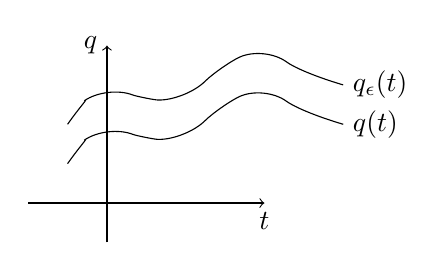
\begin{tikzpicture}[rounded corners = 10pt]
      \draw [->] (-1,0) -- (2,0) node [below] {$t$};
      \draw [->] (0,-.5) -- (0,2) node [left] {$q$};
      \draw (-.5,.5) to[bend left = 10] (0,1) to[bend right = 10] (1,.8)
        to[bend left = 10] (2,1.5) to[bend right = 10] (3,1)
        node [right] {$q(t)$};
      \draw [yshift = .5cm]
        (-.5,.5) to[bend left = 10] (0,1) to[bend right = 10]
        (1,.8)   to[bend left = 10] (2,1.5) to[bend right = 10] (3,1) node [right] {$q_\epsilon(t)$};
    \end{tikzpicture}
  \end{center}
\end{example}
\begin{example}[rotation]
  \[
    \bm q_\epsilon(t) = \bm q(t) + \epsilon \bm e_a \times q(t), \quad
    \bm f(t) = \bm e_a \times \bm q(t)
  \]
  The rotation of the world line.
  Figure: the world line rotate a angle between two time point real surface.
\end{example}
\begin{example}[time-translation]
  \[
    q_\epsilon(t) = q(t - \epsilon), \quad
    f(t) = -\dot q(t)
  \]
  \begin{center}
  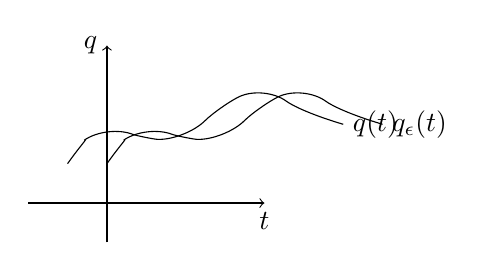
\begin{tikzpicture}[rounded corners = 10pt]
      \draw [->] (-1,0) -- (2,0) node [below] {$t$};
      \draw [->] (0,-.5) -- (0,2) node [left] {$q$};
      \draw (-.5,.5) to[bend left = 10] (0,1) to[bend right = 10] (1,.8)
        to[bend left = 10] (2,1.5) to[bend right = 10] (3,1)
        node [right] {$q(t)$};
      \draw [xshift = .5cm]
        (-.5,.5) to[bend left = 10] (0,1) to[bend right = 10]
        (1,.8)   to[bend left = 10] (2,1.5) to[bend right = 10] (3,1) node [right] {$q_\epsilon(t)$};
  \end{tikzpicture}
  \end{center}
\end{example}
For $t$-independent $\Omega_\theta$, the functional derivative
\begin{align*}
  0 & = \odv{\mathcal S[\Omega_\theta q]}\theta \bigg|_{\theta=0}
    = \frac1\epsilon (\mathcal S[\Omega_\epsilon q] - \mathcal S[q])
      \bigg|_{\epsilon \to 0}
    = \int_{t_i}^{t_f} \d t
      \ab(\pdv{\mathcal L}q \pdv{q_\theta}\theta
    + \pdv{\mathcal L}{\dot q} \pdv{\dot q_\theta}\theta) \\
    & = \int_{t_i}^{t_f} \d t
        \underbrace{\ab(\pdv{\mathcal L}q - \odv*{\pdv{\mathcal L}{\dot q}}t) f}
        _\text{E-L Equation}
      + \ab(\pdv{\mathcal L}{\dot q}f)\bigg|_{t_i}^{t_f}
\end{align*}
where we integral on shell, and
\[
  \mathcal S[q_\theta(t)] = \int_{t_i}^{t_f} \d t
  \mathcal L(q_\theta(t), \dot q_\theta(t), t)
\]
Since the E-L equation, we have
\[
  \ab(\pdv{\mathcal L}{\dot q}f)\bigg|_{t_i}^{t_f} = 0
\]
But $t_i$ and $t_f$ are arbitrary, so we can derive that
\[
  \odv*{\pdv{\mathcal L}{\dot q}f}t = 0
\]
means that it is independent from time, we get the conserved quantity.

So, in the first example $p$ is conserved; In the second one,
\[
  \mathcal S[q_\theta(t)] = \int_{t_i}^{t_f} \d t
  \mathcal L(\bm q_\theta(t), \dot{\bm q}_\theta(t), t)
\]
and
\[
  \ab(\sum_i \pdv{\mathcal L}{\dot q_i}f)\bigg|_{t_i}^{t_f} = 0
\]
so, $\bm e_a \cdot L = \bm p \cdot(\bm e_a \times \bm q(t))$
in the second example.

In the time-translation,
\[
  \mathcal S[q_\epsilon(t)] = \int_{t_i+\epsilon}^{t_f+\epsilon} \d t
  \mathcal L(q_\epsilon(t-\epsilon), \dot q_\epsilon(t-\epsilon), t)
\xlongequal{\tilde t = t - \epsilon} \int_{t_i}^{t_f} \d \tilde t
  \mathcal L(q(\tilde t), \dot q(\tilde t), \tilde + \epsilon)
\]
The derivative
\[
  0 = \odv{\mathcal S[\Omega_\theta q]}\theta \bigg|_{\theta=0}
    = \frac1\epsilon(\mathcal S[\Omega_\epsilon q] - \mathcal S[q])
    = \int_{t_i}^{t_f} \d t \pdv{\mathcal L}t \Rightarrow \pdv{\mathcal L}t = 0
\]
To interrupt it, we consider the total derivative
\[
  \odv*{\mathcal L}t = \pdv*{\mathcal L}q \dot q
+ \pdv*{\mathcal L}t\ab(\odv*{\dot q}t) + \pdv*{\mathcal L}t
\]
The second term
\[
  \pdv*{\mathcal L}t\ab(\odv*{\dot q}t)
= \odv*[fun]{\pdv{\mathcal L}q \dot q}t
- \ab(\odv*{\pdv{\mathcal L}{\dot q}}t)\dot q
\]
Substitute it and rearrange
\[
  0 = \pdv{\mathcal L}t = \odv*{\underbrace{\ab(
    \mathcal L - \pdv{\mathcal L}{\dot q} \dot q)}_\text{Hamiltonian}}t
- \underbrace{\ab(\pdv{\mathcal L}q - \odv*{\pdv{\mathcal L}q}t)}_
  \text{E-L equation} \dot q
\]
Then, we have the on-shell
\[
  \odv*{\mathcal H}t = 0
\]
i.e., the energy is conserved.

\paragraph{From (good) quantum numbers to group irrepresentation}

The statement is if
\[
  [\hat A, \hat B] = 0, \Rightarrow \exists \text{basis} \{\ket|\lambda>\}
\]
The basis vector is the eigenvector of both $\hat A$ and $\hat B$
\[
  \hat A\ket|\lambda> = \lambda_A\ket|\lambda>, \qq{and}
  \hat B\ket|\lambda> = \lambda_B\ket|\lambda>.
\]
\begin{proof}
  Consider $\hat A$ and $\hat B$ are Hermition.
  Take the ground state
  \[
    \hat A\ket|\alpha> = \alpha\ket|\alpha>
  \]
  In the case of degeneracy,
  \[
    \hat A\ket|\alpha_i> = \alpha\ket|\alpha_i>, \quad
    i = 1,\ \ldots\,,~d_\alpha
  \]
  Then, consider
  \[
    \hat A(\hat B\ket|\alpha>) = \hat B\hat A\ket|\alpha>
  = \alpha(\hat B\ket|\alpha>)
  \]
  means that
  \[
    \begin{cases*}
      \hat B\ket|\alpha> = b^{(\alpha)}\ket|\alpha>, & no-degeneracy\\
      \hat B\ket|\alpha_i> = \sum_j \ket|\alpha_j> b_{ji}^{(\alpha)}, &
      degeneracy
    \end{cases*}
  \]
  where $b_{ji}^{(\alpha)} = \braket<\alpha_j|\hat B|\alpha_i>$.
  We can always diagonalize
  \[
    b^{(\alpha_i)} = V D V^{-1}, \quad b^{(\alpha_i)} V = VD
  \]
  $D$ being a diagonal matrix $D_{ml} = \beta_l^{(\alpha)} \delta_{ml}$.
  Then,
  \[
    \sum_i b_{ji}^{(\alpha)} V_{il} = \sum_m V_{jm} D_{ml}
  = V_{jl} \beta_l^{(\alpha)}
  \]
  By take one superposition of the orginal $\alpha$
  \[
    \ket|\tilde \alpha_l> = \sum_i \ket|\alpha_i> V_{il}
  \]
  It is easy to know
  \[
    \hat B\ket|\tilde\alpha_\lambda> = \sum_i \hat B\ket|\alpha_i> V_{il}
  = \sum_{ij} \ket|\alpha_j>b_{ji}^{(\alpha)} V_{il}
  = \ket|\tilde\alpha_l> \beta_l^{(\alpha)}
  \]
  Then, the site
  \[
    \{\ket|\tilde\alpha_l>\} = \{\ket|\lambda>\}
  \]
  if there is no degeneracy, then $\ket|\tilde\alpha> = \ket|\alpha>$.
\end{proof}

\section{Symmetry group representations, degeneracies,
         inversion and time reversal}

\subsection{Group representations}

Starting from
\[
  \hat\Omega_\theta \ket|\bm r> = \ket|h_\theta(\bm r)>
\]
\begin{example}\leavevmode
  \begin{enumext}
    \item Translation $h_{\bm a} (\bm r) = \bm r + \bm r$
    \item Reflection $h_{\bm e}(\bm r) = \bm r - 2\bm r_\parallel$ (Figure required).
    \item Rotation $h_{\bm\theta = (\bm e_a, \theta)}(\bm r)
    = \bm r_\parallel + \cos\theta\bm r_\bot + \sin\theta(\bm e_a \times \bm r_\bot)$.
  \end{enumext}
  For an arbitary state $\ket|\psi>$, how the operator act on the arbitary state
  \[
    (\hat\Omega_\theta\psi)(\bm r)
  = \braket<\bm r|\hat\Omega_\theta|\psi>
  = \braket<h_\theta^{-1}(\bm r)|\psi> = \psi(h_\theta^{-1}(\bm r))
  \]
  Then, consider a general
  \[
    (\hat\Omega_2\hat\Omega_1\psi)(\bm r)
  = \braket<\bm r|\hat\Omega_2\hat\Omega_1|\psi>
  = \braket<h_2^{-1}(\bm r)|\Omega_1\psi>
  = \braket<(h^{-1}h_2^{-1})(\bm r)> \ket|\psi>
  \]
  where we can treat $\hat\Omega_2\hat\Omega_1 = \hat\Omega_3$.
  The transformation converses the distance $\bm r_1 - \bm r_2$,
  then, all the $h$
  \[
    h(\bm r_1 - \bm r_1) = |h(\bm r_1) - h(\bm r_1)| = |\bm r_1 - \bm r_2|
  \]
  form the Euclidian space (Group)
  \begin{equation}
    E(d):\ \{h||h(\bm r_1 - \bm r_2) = |\bm r_1 - \bm r_2|\}
  \end{equation}
  \begin{enumext}
    \item All the translation form $T(d)$
    \item All the reflection form $O \in \text{reflection place}$
    \item All the rotationform $O(d)$, orthogonal group.
  \end{enumext}
  But, in Euclidian space, it will become a semi-direct product
  \[
    T_d \rtimes O(d)
  \]
  where $O(d) = \text{SO}(d) \times \mathbb Z_2$ is orthogonal.
  For $\{M_d:\ M^\dagger M = \identity\}$, then $(\det(M))^2 = 1$,
  $\det(M) = \pm 1$. This means that $S$ can be special for $\det(M) = +1$.
  While $Z_2$ have two $\{+1, -1\}$.
\end{example}

We have a Euclidian group
$\{\hat\Omega_\theta\} \leftarrow G = E(d) \to \{h_\theta\}$ corresponding to
all the operators.
\begin{equation}
  \overset{\mathbb V = \{\ket|\bm r>\}}
    {\underset{(G\circlearrowright\mathbb V)}{\{\hat\Omega_\theta\}}}
  \xlongleftarrow[\substack{
    \Omega_1\mapsfrom g_1,\ \Omega_2\mapsfrom g_2\\
    \Omega_1\Omega_2 \mapsfrom g_1 \cdot g_2
  }]{\text{homomorphism}}
  \underset{\substack{\rotatebox{90}{$=$}\\E(d)}}{G}
  \xlongrightarrow{\text{homo}}
  \overset{\mathbb R = \{\bm r\}}
    {\underset{(G\circlearrowright\mathbb R^d)}{\{\hat h_\theta\}}}, \quad
  G \longrightarrow GL(V), \quad \Omega: V \to V
\end{equation}
where ``homomorphism'' means the same shape and form,
$h_\theta$ acts on $\bm r$ while $\hat\Omega_\theta$ acts on $\ket|\bm r>$.
They form \emph{Group Action}: Representation.

\paragraph{Translation group}

We start from the translation group $T(d)$. Consider
\[
  T_{\bm a} \cdot T_{\bm b} = T_{\bm a + \bm b = \bm b + \bm a}
\]
we call it the \emph{Abelian Group}.
In Hilbert space of this case, $V = \operatorname{span}(\{\ket|\bm r>\})$.
Then, the operator $\hat T_{\bm a}$ on this space
\[
  \hat T_{\bm a} = \upe^{-\iu\bm a\cdot\hat{\bm k}}
\]
where $\hat g_{T_i} = \hat k_i$ for $i = 1$, $2$, $3$.
\paragraph{Quiz}
Now, consider
\[
  T_{\bm a} \xlongequal{k\to\iu\nabla} \upe^{-\bm a \cdot\nabla}
\]
Calculate
\[
  \braket<\bm r|\hat T_a|\psi> = (T_{\bm a}\psi)(\bm r)
= \psi(\bm r - \bm a).
\]
By Foruier transform , where one can have the eigenvalue Equation
\[
  \nabla \upe^{\iu\bm k\cdot\bm r} = -\iu \bm k \upe
\]
and in Foruier transform
\[
  \psi(\bm r) = \int \d\bm k \tilde\psi(\bm k) \upe^{\iu\bm k\cdot\bm r}
\]
we can have
\[
  f(\nabla) \upe^{\iu \bm k\cdot\bm r} = f(\iu\bm k) \upe^{\iu\bm k\cdot\bm r},
  \quad
  \upe^{-\bm a\cdot\nabla} \upe^{\iu\bm k\cdot\bm r}
= \upe^{\iu\bm k\cdot(\bm r-\bm a)}
\]
Due to the property of the transform operator
\[
  \upe^{-\bm a\cdot\nabla} \psi(\bm r) = \psi(\bm r - \bm a)
\]
substitute the identities above
\[
  \upe^{-\bm a\cdot\nabla} \psi(\bm r)
= \int \d\bm k \tilde\psi(\bm k) \upe^{\iu\bm k(\bm r-\bm a)}
= \psi(\bm r - \bm a)
\]
\rule{\linewidth}{1pt}
For Abelian group, we have the commutative generator
\[
  [\hat k_i, \hat k_j] = 0
\]
\begin{enumext}
  \item $V = \{\ket|\bm k, \sigma>|\hat{\bm k} \ket|\bm k,
    \sigma> = \bm k\ket|\bm k, \sigma>, \bm k \in \mathbb R^3\}$.
  Now, the Hilbert space becomes a direct sum
  \[
    V = \bigoplus_{\bm k\in\mathbb R^3} V_{\bm k}, \qq{where}
    V_{\bm k_0} = \operatorname{span}(\{\ket|\bm k_\sigma, \sigma>\})
  \]
  \item $[\hat H, \hat{\bm k}] = 0$, $\forall \bm a$. The Hamiltonian operator
  also becomes
  \[
    \hat H = \bigoplus_{\bm k\in\mathbb R^3} \hat H_{\bm k}
  = \pdiagmat[empty = {}]{H_{\bm k_1}, H_{\bm k_2}, \ddots}
  \]
  where
  \[
    \hat H_{\bm k} = P_{\bm k} \hat H P_{\bm k}, \qq{and}
    P_{\bm k} = \sum_\sigma \ketbra|\bm k,\sigma><\bm k, \sigma|
  \]
  Then, $V_{\bm k} = P_{\bm k}V$, the so-called \emph{Bloch Theorem}\footnote{%
    In the lattice, we need to change $\bm a \in \mathbb R^3 \to \mathbb Z^3$}.
\end{enumext}

\paragraph{Non-abelian Group}

\begin{example}
  $\text{SO}(d)$ for $d > 2$
\end{example}
\begin{example}[Dihedred Group for $n$-gon]
  The elements
  \[
    \{e,\ R,\ R^2, \rho_0, \rho_1,\ \rho_2\} = \bra<R,\rho = \rho_0|
    \qq{(generators)}
  \]
  where
  \begin{enumext}[columns = 2]
    \item $R^2 = \bar R$
    \item $\rho_i = \bar\rho_i$
    \item $R^3 = e = \rho_i$
    \item $R\rho_i\bar R = \rho_{i+1}$
    \item $\rho R \bar\rho_0 = \bar R$
  \end{enumext}
  In summary
  \begin{enumext}[columns = 2]
    \item $R\rho_0\bar R = \rho_{R(0)}$
    \item $\rho_0 R\bar\rho_0 = R_\text{flip} = \bar R$
    \item $\rho_i\rho_{i+1} = R$
    \item $\rho_{i+1}\rho_i = \bar R$
  \end{enumext}
  From $\rho_a\rho_b = T_{2(a+b)}$, we have
  \[
    \rho_i \rho_{i\pm 1} = T_{\mp2} = T_{\pm 1} = R^2
  \]
  and from $\rho_a\rho_b\rho_c = \rho_{a-b+c}$, we have
  \[
    \rho_0\rho_1\bar\rho_0 = \rho_{0-1+0} = \rho_{-1} = \rho_2
  \]
  \[
    R\rho_0 = \rho_2 \rho_0 \rho_0 = \rho_2, \quad
    R^2 \rho_0 = \rho_1
  \]
\end{example}
Cayley Table (Group Multiplication Table)
\[
  \{e,\ R,\ R^2, \rho_0, \rho_1,\ \rho_2\} = \braket<\underbrace{R,\rho = \rho_0}_\text{generators}|
  \underbrace{R^3 = \rho^2 = e, \rho R = R^2\rho}_\text{relations}>
\]
where $R^{n_1}$, $\rho^{m_1}$, $R^{n_2}$, $\rho_{m_2}$
will appear in the group. We can always switch $R$ and $\rho$ since
\[
  \rho R = R^2 \rho
\]
Similar for $D_n$.

Now, we can define two operators
\[
  \hat R\ket|i> = \ket|R(i)> = \ket|i + 1>, \qq{and}
  \hat\rho\ket|i> = \ket|\rho(i)> = \ket|-i>
\]
on Hilbert space $V = \operatorname{span}(\{\ket|0>, \ket|1>, \ket|2>\})$.
The Hamiltonian
\[
  \hat H = \sum_{i,j = 0,1,2} \ketbra|i> h_{ij} <j|
\]
where $h_{ij} = h_{ji}^*$. So,
\[
  \forall \hat g \in D_3,\ [\hat H, \hat g] = 0 \Rightarrow ?
\]
Since $\hat R\hat H\hat R^{-1} = \sum_{ij} \ketbra|i+1>h_{ij}<j+1| = \hat H$, then
\[
  h_{ij} = h_{i+1,j+1}, \quad
  h_{ij} = h_{-i, -j}
\]
we have
\[
  \hat H = \begin{pmatrix}
    \epsilon & t & t\\ t& \epsilon & t\\t & t' & \epsilon
  \end{pmatrix} =
  \begin{pmatrix}
    0 & t  & t\\
    t & 0  & t\\
    t & t' & 0
  \end{pmatrix}
\]
The eigenvalue and eigenvector, the basis are $\ket|0>$, $\ket|1>$, $\ket|2>$.
\[
  \hat H = t(\hat R + \hat R^2)
\]
we know $\hat R^3 = 1$, then the eigenvalue should be
$\lambda_n = \upe^{\iu\frac{2\pi}3}$
\[
  \hat R\ket|\psi_n> = \upe^{\iu\frac{2\pi}{3}n} \ket|\psi_n>, \quad
  n = 0,\ 1,\ 2
\]
Then eigenvalues are
\[
  E_{\psi_0} = 2t, \quad E_{\psi_1} = E_{\psi_2} = t(\omega + \omega^*)
\]
we arrive at the degeneracy.

\subsection{Degeneracies}

Now, write the operators $\hat R$ and $\hat \rho$ into the basis
\[
  \{\ket|\psi_0>,\ \ket|\psi_1>,\ \ket|\psi_2>\}
\]
$R_\psi$ in the $\psi$ basis, it is diagonal
\[
  R_\psi = \pdiagmat{1, \omega, \bar\omega}
\]
Calculate how $\hat R(\hat\rho\ket|\psi_0>)$ acts.
\[
  \hat R(\hat\rho\ket|\psi_0>) = \hat\rho \hat R^2 \ket|\psi_0>
\xlongequal{\hat R\ket|\psi_0> = \ket|\psi_0>} \hat\rho\ket|\psi_0>
\]
So, $\braket<\psi_i|\hat\rho|\psi_0> = \delta_{i,0}$.
For $\ket|\psi_1>$,
\[
  \hat R(\hat\rho\ket|\psi_1>) = \hat\rho \hat R^2 \ket|\psi_1>
= \bar\omega \hat\rho \ket|\psi_1>
\]
So, in matrix
\[
  R_\psi = \begin{pmatrix}
    1 & & 0\\
    & \omega\\
    0 & & \bar\omega
  \end{pmatrix}, \quad
  \rho_\psi = \begin{pmatrix}
    1 & 0\\
    0 & & 1\\
    & 1
  \end{pmatrix}
\]
In the new basis, the Hilbert space
\[
  V = V_{\psi_0} \oplus V_{\{\psi_1, \psi_2\}}, \quad
  g = g_{\psi_0} \oplus g_{\{\psi_1,\psi_2\}}
\]
and
\[
  0 = \braket<\psi_1|\hat\rho|\psi_1>
\]
This is why the degeneracy occurs.
\[
  \hat H\ket|\psi> = E\ket|\psi>, \quad
  \hat H(\hat\rho\ket|\psi>) = \hat\rho \hat H\ket|\psi>
= E(\hat\rho\ket|\psi>).
\]

\paragraph{Quick Review of Group Representation}

Starting from
\[
  \underset{\text{Group}}G
  \overset{\tau}{\underset{\text{acts on}}{\circlearrowright}}
  \underset{\text{linear space}}V, \quad
  \tau:\ G \rightarrow
  \underset{\text{Linear operator space on $V$}}
    {\overset{\text{opened}}G\overset{\text{linear}}L(V)}
\]
where $\tau$ is homomorphism:
\[
  \forall \underset{\rotatebox{-90}{$\mapsto A_{1,2}$}}{g_{1,2}} \in G, \quad
  (g_1 \circ g_2) \longmapsto A_1 A_2
\]

\begin{example}
  For the group $D_3 = \{e, R, R^2, \rho_0, \rho_1, \rho_2\} \cong S_3$
  which satisfy $R^3 = \rho^2 = e,\ R\rho = \rho R^2$.
  \begin{paracol}{2}
    \[
      (\quad),\ (012) = (120) = (201),\ (021),\ (12),\ (20),\ (01)
    \]
    For example, $(12)(12) = (\quad)$, $(012)(12) = (10)$.
    \switchcolumn \centering
    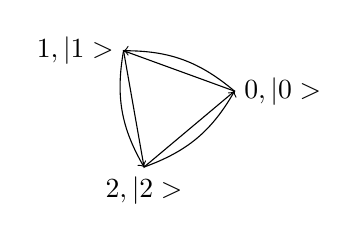
\begin{tikzpicture}[scale = 1.5]
      \draw [rotate = 10] (0,0) coordinate (a)
       node [left] {$1, \ket|1>$} -- (0,-1) coordinate (b)
       node [below] {$2, \ket|2>$} -- ({sqrt(3)/2},-.5)
       coordinate (c) node [right] {$0, \ket|0>$} -- cycle;
      \draw [->] (c) to[bend right = 20] (a);
      \draw [->] (a) to[bend right = 20] (b);
      \draw [->] (b) to[bend right = 20] (c);
    \end{tikzpicture}
  \end{paracol}
  Then, for the group multiplication
  \[
    (12)(012) = (12)(120) = (12)(12)(20) = (20), \quad
    (12)(021) = (12)(210) = (12)(21)(10) = (10)
  \]
  Consider taking $i \mapsto \ket|i>$, basis of Hilbert space $V$
  ($\{\ket|0>, \ket|1>, \ket|2>\}$). Then, the identities become
  \[
    \hat R\ket|i> = \ket|R(i)>,   \quad
    \hat R\rho\ket|i> = \ket|\rho(i)>.
  \]
  Then, we can say $\{e, R, R^2, \rho_0, \rho_1, \rho_2\} \subset V$.
  The Hilbert space can be composed into two parts
  \[
    V = V_{\psi_0} \oplus V_{\{\psi_1,\psi_2\}}
  \]
  where $\ket|\psi_n>$ means $\hat R\ket|\psi_n> = \omega^n \ket|\psi_n>$,
  $\omega = \upe^{\iu\frac{2\pi}{3}}$.
  So, the subspace
  \[
    V_{\psi_0} = \operatorname{span}(\{\psi_0\}),\
    V_{\{\psi_1,\psi_2\}} = \operatorname{span}(\{\psi_1,\psi_2\})
  \]
  $\forall \hat g \in \hat D_3$,
  \[
    g =
    \begin{pNiceArray}{c|cc}[first-col, last-row]
      \ket|\psi_0> &
      \Block[tikz = {pattern = north east lines, pattern color = teal}]{}{}
      & \Block{1-2}{O}\\
      \hline
      \ket|\psi_1> & \Block{2-1}{O} &
      \Block[tikz = {pattern = north east lines, pattern color = teal}]{2-2}{}\\
      \ket|\psi_2> & \\
    & \bra<\psi_0| & \bra<\psi_1| & \bra<\psi_2|
    \end{pNiceArray}
  \]
  where the generator
  \[
    R = \begin{pNiceArray}{c|cc}
      1 & \Block{1-2}{O}\\
      \hline
      \Block{2-1}{O} & \omega\\
      & & \omega^*
    \end{pNiceArray}, \quad
    \rho = \begin{pNiceArray}{c|cc}
      1 & \Block{1-2}{O}\\
      \hline
      \Block{2-1}{O} & & 1\\
      & 1
    \end{pNiceArray}
  \]
  we label the subspace $V_{\psi_0}$ as $A_1$, and label $V_{\{\psi_1,\psi_2\}}$
  as $E$. Then
  \[
    e_A = 1,\quad R_{A_1} = 1, \quad \rho_{A_1} = 1 \Rightarrow g_{A_1} = 1,
  \]
  \[
    e_E = \pdiagmat[empty = {}]{1,1},\quad
    R_E = \pdiagmat[empty = {}]{\omega, \omega^*}, \quad
    \rho_E = \begin{pmatrix}
      & 1\\1
    \end{pmatrix} \text{(Equivalent Representations)}
  \]
  The multiplication
  \[
    R_E \rho_E = \begin{pmatrix}
      0 & \omega \\ \omega^* & 0
    \end{pmatrix} = \rho_E R_E^2 = \begin{pmatrix}
      & \omega \\\omega^*
    \end{pmatrix} \pdiagmat[empty = {}]{\omega^*, \omega}.
  \]
  For non-Abelian group, $\hat R\hat \rho \neq \hat \rho \hat R$.
  \[
    \text{\underline{minimal} invariant subspace} \leftrightarrow
    \text{\underline{irreducible} (sub)representation}
  \]
\end{example}
Now, consider the Hilbert space becomes
\[
  \operatorname{opan}(\{\ket|0\pm>, \ket|1\pm>, \ket|2\pm>\}).
\]
Induce
\[
  i \pm \mapsto \ket|i\pm>, \quad
  \hat R\ket|i,s> = \ket|i+1,s>,\
  \hat\rho \ket|i,s> = \ket|-i,-s>
\]
Consider the Hamiltonian
\[
  \hat H = \sum_{j,s,j',s'} \ketbra|j,s>h_{js;j's'} <j's'|
\]
which satisfies
\[
  [\hat R, \hat H] = [\hat\rho, \hat H] = 0
\]
\[
  \begin{array}{c}
    \{\text{Transformations on Real Space}\}\\
    \text{def} \downarrow \uparrow \text{represent}\\
    G\\
    \downarrow \text{represent}\\
    \{\text{Transformations on
      $\underset{\text{HS $V$ represent}
        \{\text{Transformations on Operator Space}\}}
        {\text{Function Space}}$}\}, \quad \{V \to V\}
  \end{array}
\]
For invariant subspace $W$ (group action):
$\forall g \in G$, $\ket|w> \in W$, we have
\[
  \hat g (= \tau(g)) \ket|w> \in W
\]
Now, minimal invariant subspace $\leftrightarrow$ irreducible representation.
Choose $\ket|\psi_1>$, which satisfies
\[
  \hat H\ket|\psi_1> = E\ket|\psi_1>
\]
Then, $\ket|\psi_2> = \hat\rho\ket|\psi_1>$, and they are orthogonal to each
other $\braket<\psi_2|\psi_1> = 0$, then
\[
  \hat H \hat \rho \ket|\psi_1> = E\hat \rho \ket|\psi_1>
\]
\paragraph{Schur's Lemma}
In irrepresentation $\tau$, if $[\hat H_\tau, \hat g_\tau] = 0$
$\forall g \in G$, then it is the irrepresentation of $G$.
Then, $\hat H_\tau = E\identity_\tau$,
which call $\dim(V_\tau) = \#\text{Degeneracy}$.

\paragraph{Space Inversion \& Time Reversal}

\begin{center}
  \begin{minipage}[t]{.64\linewidth}
    \centering
    \begin{tabular}{*3l}
      \toprule
      Classical & $\mathcal I = \rho_x \rho_y \rho_z$ & $\mathcal T$\\
      \midrule
      & $\bm r \to -\bm r$, $t \to t$ &
      $t \to -t$, $\bm r \to \bm r$\\
      & $\bm p \to -\bm p$ & $\bm p \to -\bm p$\\
      \midrule
      Polar (Vector) & $\bm E \to -\bm E$ & $\bm E \to \bm E$\\
      Axial (Pseudo vector) & $\bm B \to \bm B$ & $\bm B \to -\bm B$\\
      $\bm E = -\nabla\varphi$ & $\varphi \to \varphi$ & $\varphi \to \varphi$\\
      $\bm A = \nabla \times \bm B$ & $\bm A \to -\bm A$ & $\bm A \to \bm A$\\
      \bottomrule
    \end{tabular}
  \end{minipage} \hfill
  \begin{minipage}[t]{.32\linewidth}
  Quantum:

  \begin{tabular}{ll}
    \toprule
    $\hat I$ & $\hat T$\\
    \midrule
    $\hat I \hat{\bm r} \hat I^{-1} = -\hat{\bm r}$ &
    $\hat T\hat{\bm r}\hat T^{-1} = \hat{\bm r}$\\
    $\hat I \hat{\bm p} \hat I^{-1} = -\hat{\bm p}$ &
    $\hat T\hat{\bm p}\hat T^{-1} = -\hat{\bm p}$\\
    $\hat I[\hat x, \hat p_x]\hat I^{-1} = [-\hat x, -\hat p_x] = \iu$ &
    $\hat T[\hat x, \hat p_x]\hat T^{-1} = [\hat x, -\hat p_x] = -\iu$\\
    \bottomrule
  \end{tabular}
  \end{minipage}
\end{center}

For $\hat f$ anti-linear
\[
  \hat f(a\ket|\psi> + b\ket|\chi>
= a^*\hat f\ket|\varphi> + b^*\hat f\ket|\chi>)
\]
Norm-preserving
\[
  \braket<\hat f\psi|\hat f\psi> = \braket<\psi|\psi>
\]
\paragraph{Quiz}
Prove that $\forall \psi,\ x_i$,
$\braket<\hat f\psi|\hat f\chi> = \braket<x|\psi> = \braket<\psi|\chi>^*$.
BTW, when it is satisfied, $f$ is called anti-unitary.

We already have
for $\hat I$: $\{e, I\}$, $I^2 = e$;
and for $T$: $\{e,T\}$, $T^2 = e$.
Combine irreps of $\{e,i\}$, and $i^2 = e$ called involution.
\[
  \ket|\psi> \sim \upe^{\iu\theta}\ket|\psi> \in V,
\]
then
\[
  \hat e\ket|\psi> = \ket|\psi>, \quad
  \hat i\ket|\psi> = \ket|\chi>, \quad
  \hat i^2 \ket|\psi> = \hat i \ket|\chi> = \upe^{\iu\theta} \ket|\psi>.
\]
Take $\ket|\chi> \propto \ket|\psi>$, then $\braket<\psi|\chi> = 0$.
Start with $\hat i$ be unitary with $\hat I$ is unitary.
We can always construct another state with a linear combination
\[
  \ket|\phi> = a\ket|\psi> + b\ket|\chi>,
\]
Then,
\[
  \ket|\phi> \propto \hat i_\pm\ket|\phi> = a_\pm\ket|\chi> + b\upe^{\iu\theta}\ket|\psi>
\]
Rearrange it
\[
  \frac{b\upe^{\iu\theta}}{a} = \frac ab, \quad
  \ab(\frac ab)^2 = \upe^{\iu\theta}, \quad
  g = 1,\ a_\pm = \pm \upe^{\iu\theta}
\]
For anti-unitary, we need to
\[
  \ket|\phi> \propto \hat i\ket|\phi>
= a^*\ket|\chi> + b^*\upe^{\iu\theta}\ket|\psi>
\]
Rearrange it
\[
  \frac{b^* \upe^{\iu\theta}}{a} = \frac{a^*}{b} \Rightarrow
  |a|^2 = |b|^2\upe^{\iu\theta}
\]
If $|a|^2 = |b|^2$, $\upe^{\iu\theta} = 1$.

\subsection{Propective Representation}

The unitary operator $\hat I$ and anti-unitary operator $\hat T$.
The homomorphism $\rho:\ G \to GL(V)$.
\[
  \forall g, h \in G, \rho(g) \rho(h) \sim \rho(gh)
\]
In quantum mechanics, we are allowed to have a global phase
\[
  \rho(gh) = \upe^{\iu\theta(gh)} \rho(g) \rho(h)
\]
This phase factor is basically the constraints of $\theta$ by consistency
\[
  \rho(ghk) = \begin{cases}
    \upe^{\iu\theta(g,hk)} \rho(g) \rho(hk)
  = \upe^{\iu(\theta(g,hk) + \theta(h,k))} \rho(g) \rho(h) \rho(k)\\
    \upe^{\iu\theta(gh, k)} \rho(g,h) \rho(k)
  = \upe^{\iu(\theta(gh,k) + \theta(g,h))} \rho(g) \rho(h) \rho(k)\\
  \end{cases}
\]
The two factors should the same, then
\[
  \theta(g,hk) + \theta(h,k) \cong \theta(gh,k) + \theta(g,h)
\]
which is the so-called cocycle condition.
\begin{enumext}
  \item If $\theta = 0$, we arrive at the linear representations.
  \item Suppose for any $\theta$, $g$, and $h$
  \[
    \delta \theta_\phi(g,h) = \phi(g) + \phi(h) - \phi(gh)
  \]
  Then, the cocycle condition becomes
  \[
    \phi(g) \cancel{+ \phi(hk)} - \phi(ghk) + \phi(h) + \phi(k)
    \cancel{-\phi(hk)}
  \]
  is automatically satisfied. Given $\forall g$, $h \in G$
  \[
    \tilde\theta(g,h) = \theta(g,h) + \delta \theta_\phi(g,h)
  \]
  where the cocycle condition always satisfied. So
  \[
    \tilde \theta \sim \theta
  \]
  The equivalence is eventually related to topology.
\end{enumext}
Consider 4 $\theta$s for the group $\mathbb Z_2 = \{e, g\}$, where $g^2 = e$,
and $g$ can be time-invariant $\hat I$ or space-invariant $\hat T$
\[
  \theta(e,e) = \theta(e,g) = \theta(g,e) = 0,\quad
  -\theta := \theta(g,g), \quad
  \hat g^2 = \upe^{\iu\theta} \identity.
\]
$\rho(e) = \identity$ is always true, the three ones are numbers, while the last
one is a function. For arbitary state $\ket|\psi>$
\[
  \hat g \ket|\psi> = \ket|\chi>, \quad
  \hat g \ket|\chi> = \hat g^2 \ket|\psi> = \upe^{\iu\theta} \ket|\psi>
\]
\begin{enumext}
  \item $\hat g$ is unitary
  \[
    \hat g(\ket|\psi> \pm \upe^{-\iu\theta/2} \ket|\chi>)
  = \ket|\chi> \pm \upe^{+\iu\theta/2} \ket|\psi>
  = \pm \upe^{\iu\theta/2} (\ket|\psi> \pm \upe^{-\iu\theta/2} \ket|\chi>)
  \]
  we obtain the eigenvectors of $\hat g$:
  $\ket|\psi> \pm \upe^{-\iu\theta/2} \ket|\chi>$, 1D irreducible
  representation, all equivalent.

  The phase factor can be absorbed into $\hat g$.
  \item $\hat g$ is anti-unitary: using the same trick.
  \[
    \hat g(a\ket|\psi> + b\ket|\chi>) = a^*\ket|\psi>
  + b^*\upe^{\iu\theta} \ket|\psi>
  \]
  Note: For anti-unitary operator, when the scalor $a$ and $b$ pass through it,
  it should take the conjugate. Where the factors should satisfy
  (we obtained before)
  \[
    \frac a{b^*\upe^{\iu\theta}} = \frac b{a^*} \Rightarrow
    |a|^2 = |b|^2\upe^{\iu\theta}
  \]
  \begin{enumext}
    \item $\hat T^2 = \upe^{\iu\theta} = +1$: eigenvector becomes 1D irreducible
    representation.
    \item $\hat T^2 = \upe^{\iu\theta} \neq +1$, then no eigenvector possible, it has to be
    2D irreducible representation basically in the space of
    $\{\ket|\psi>, \ket|\chi>\}$.
  \begin{remark}[Constraint on $\upe^{\iu\theta}$]
    \[
      \hat g^3 \ket|\psi> =
      \begin{cases}
        \hat g^2 (\hat g(\ket|\psi>)) = \upe^{\iu\theta} (\hat g\ket|\psi>)\\
        \hat g (\hat g^2 \ket|\psi>) = \upe^{-\iu\theta} (\hat g\ket|\psi>)
      \end{cases} \Rightarrow \upe^{\iu\theta} = \pm 1
    \]
    This ``magic'' happens due to the fact that \emph{$\hat g$ is anti-unitary}.
    So, the second point (ii) becomes
  \end{remark}
  \item $\hat T^2 = \upe^{\iu\theta} = -1$, then no eigenvector possible, it has
  to be 2D irreducible representation basically in the space of
  $\{\ket|\psi>, \ket|\chi>\}$.
  \end{enumext}
\end{enumext}
Put these into context, for the time-inversal operator,
$\hat T^2 = \pm \identity$.
\begin{enumext}
  \item Consequence of $\hat T^2 = -1$
  \[
    O = \braket<\psi|\hat T\psi> = \braket<\psi|\chi>
  = \braket<\chi|\psi>^* = \braket<\hat T\chi|\hat T\psi>
  \xlongequal{\hat T^2\psi = -\psi, \hat T\psi = \chi} -\braket<\psi|\chi>
  \]
  This is the so-called Kramers pair.
  \item Time-Reversal \underline{Symmetry}
  \[
    [\hat T, \hat H] = 0
  \]
  \begin{enumext}
    \item $\hat T^2 = +1$
    In the basis of $\{\ket|\alpha>, \hat T\ket|\alpha> = \ket|\alpha>\}$
    \[
      \hat T\ket|\alpha> = \upe^{\iu\phi(\alpha)} \ket|\alpha>, \quad
      \ket|\tilde\alpha> = \upe^{\iu\phi_\alpha/2} \ket|\alpha>,\quad
      \hat T\ket|\tilde\alpha> = \upe^{-\iu\phi_\alpha/2}
      \upe^{\iu\phi_\alpha} \ket|\alpha>
    \]
    means $\ket|\tilde\alpha>$ all matrix elements of $\hat H$ are real.
    \[
      \hat T = K \qq{complex comjugation} \Rightarrow
      H_{\alpha\alpha}^* = H_{\alpha\alpha}
    \]
    From $[\hat T, \hat H] = 0$, we can obtain
    $\hat H = \hat T\hat H\hat T^{-1}$.
    \item $\hat T^2 = -1 \to $ 2D irreducible representation $\to$ basis
    \[
      \{(\ket|\alpha_n>, \ket|\beta_n>),
      \hat T\ket|\alpha_n> = \ket|\beta_n>,
      \hat T\ket|\beta_n> = -\ket|\alpha_n>\}
    \]
    satisfies block diagonal $\hat T$
    \[
      \hat T = \theta_n \begin{pmatrix}
        & -1\\1
      \end{pmatrix} K = (-\iu\sigma_y) K
    \]
  \end{enumext}
\end{enumext}
\paragraph{Quiz2}
Starting with $\hat T\hat H \hat T^{-1} = \hat H$ (or $[\hat T, \hat H] = 0$).
In the Hilbert space $V = \oplus_n V_n$,
where $V_n = \operatorname{span} (\{\ket|\alpha_n>, \ket|\beta_n>\})$.

Substitute $\hat T$
\[
  \begin{pmatrix}
    & -1\\1 &
  \end{pmatrix} H_{nn'}^* = H_{nn'} \begin{pmatrix}
    & -1\\1
  \end{pmatrix}
\]
where the equation of $H_{nn'}$ satisfies
\begin{CJK*}{UTF8}{bsmi}
\[
\begin{pmatrix}
  -\text{丙} & -\text{丁}\\
  \text{甲} & \text{乙}
  \end{pmatrix} = 
  \begin{pmatrix}
    & -1\\1
  \end{pmatrix}
  \begin{pmatrix}
    \text{甲}^* & \text{乙}^*\\
    \text{丙}^* & \text{丁}^*\\
  \end{pmatrix} =
  \begin{pmatrix}
    \text{甲} & \text{乙}\\
    \text{丙} & \text{丁}\\
  \end{pmatrix}
  \begin{pmatrix}
    & -1\\1
  \end{pmatrix} =
  \begin{pmatrix}
    \text{乙} & -\text{甲}\\
    \text{丁} & -\text{丙}
  \end{pmatrix}
\]
Then, we have
\[
  \begin{cases}
    \text{甲} = \text{丁}^*,\\
    \text{乙} = -\text{丙}^*
  \end{cases}, \quad
  \text{甲} = a + \iu d, \quad
  \text{乙} = c + \iu b.
\]
Then, we can express $H_{nn'}$ as
\[
  H_{nn'} =
  \begin{pmatrix}
    \text{甲} & \text{乙}\\
    -\text{乙}^* & \text{甲}
  \end{pmatrix} = a\sigma_0 + d(\iu\sigma_z) + b(\iu\sigma_x) + c(\iu\sigma_y)
\]
which means $H_{nn'}$ is quaternion.
\end{CJK*}
In the second sequence,
\[
  \hat H\ket|\psi> = E\ket|\psi>, \quad
  \hat H(\hat T\ket|\psi>) = \hat T\hat H\ket|\psi>
= E(\hat T\ket|\psi>).
\]
So-called Kramers-Dageneracy.

\paragraph{Experiment}
Given $\hat T^2 = -1$, means do it twice, and there will two twists on the
world-line (ribbon); for $(\hat T^2)^2 = +1$, turn the ribbon for 4 times, then
let one point pass through under the other part of the ribbon, it restores to
the original plain one.

\section{Angular momentum, Lie algebra}

\subsection{SO(3) / SU(2) groups}

The SO(3) group is rotations in 3D, SU(2) group: innerspace.
\begin{definition}[Rotations in 3D]
  For $v \in \mathbb R$,
  \[
    (Rv)\tran (Rv) = v\tran v, \Rightarrow R\tran R = \identity_3, \quad
    \det R = +1, \quad (\det R)^2 = 1
  \]
  means the group can be defined as
  \[
    \text{SO(3)} = \{R:\ R\tran R = \identity_3,\ \det R = +1\}
  \]
  One can also consider the operator $R = \upe^A$, where $A\tran = -A$
  \[
    A = \begin{pmatrix}
      0 & \theta_3 & -\theta_2\\
      -\theta_3 & 0 & \theta_1\\
      \theta_2 & -\theta_1 & 0
    \end{pmatrix} = \sum_{a = 1,2,3} \theta_a(ij_a)
  \]
  where $(j_a)_{bc} = (-\iu)\epsilon_{abc}$,
  $ij_a = \pdv{R(\bm\theta)}{\theta_a}\bigg|_{\bm\theta = 0}$.
  \[
    ij_1 = \begin{pmatrix}
      0 & \\&
      & 1\\ & -1
    \end{pmatrix},\quad
    ij_2 = \begin{pmatrix}
      & & -1\\
      & 0\\1
    \end{pmatrix},\quad
    ij_3 = \begin{pmatrix}
      & 1\\
      -1\\
      & & 0
    \end{pmatrix}
  \]
\end{definition}
\begin{definition}
  \[
    \text{SU(2)} = \{U, (Uv)^\dagger (Uv) = v^\dagger v,\
    U^\dagger U = \identity_2,\ \det U = +1\}
  \]
  where $v \in \mathbb C^2$. For
  \[
    U = \upe^{\iu H},\quad H^\dagger = H, \quad
    H = \sum_a \theta_a \frac{\sigma_a}{2}.
  \]
  Substitute $H$ into $U$
  \[
    U(\bm\theta) = \upe^{\iu\sum_a \theta_a \frac{\sigma_a}{2}}
  \]
  $\sigma$ here are Pauli matrices.
  \paragraph{Quiz}
  \begin{enumext}[columns = 3]
    \item $[j_1, j_2] = ij_3$
    \item $[\frac{\sigma_1}{2}, \frac{\sigma_2}{2}] = \iu\frac{\sigma_3}{2}$
    \item $[\hat L_1, \hat L_2] = \iu\hat L_3$
    \item $[j_a, j_b] = \iu\epsilon_{abc} j_c$
    \item $[\frac{\sigma_a}{2}, \frac{\sigma_b}{2}] = \iu\epsilon_{abc} \frac{\sigma_c}{2}$
    \item $[\hat L_a, \hat L_b] = \iu\epsilon_{abc} \hat L_c$.
  \end{enumext}
\end{definition}

\subsection{Lie algebra}

Algebra is vector space, we define vector product
\[
  \qq{bilinear:} V \times V \to V, \quad
  V = \operatorname{span}(\{g_a\})
\]
A generator is something similarly to
\[
  g_a = \pdv{U(\bm \theta)}{\theta_a} \bigg|_{\bm\theta = 0}
\]
Lie bracket $[\cdots]$
\[
  \qq{Antisymmetric} [u, v] = -[v, u]
\]
and Jacobi identity
\[
  [u,[v,w]] + [v,[w,u]] + [w,[u,v]] = 0
\]

\section{Theory of Angular Momentum (Theory of Irreps of SO(3) Lie Algebra)}

The Lie bracket
\[
  [\quad, \quad]: (a,b) \mapsto [a,b]
\]
It satisfy two properties
\begin{enumext}
  \item Anti-symmetry: $[a,b] = -[b,a]$, which concerns the ``commutativity''.
  \item Jacobi's identity: $[a, [b,c]] + (bca) + (cab) = 0$, which concerns
  the ``associativity''.
\end{enumext}
Lie Algebra $(V,[,])$ contains: The tangent space of the Lie group,
and its product.
\[
  V = \operatorname{span} (\{g_a\}), \quad
  g_a = \iu \pdv{\Omega_q}{\theta_a} \bigg|_{\theta = 0} = 0.
\]
For any $a$ and $b$
\[
  [g_a, g_b] = \iu f_{abc}g_c
\]
where $f_{abc}$ is the structure constant.
We define
\begin{equation}
  J_\pm = J_1 \pm \iu J_2
\end{equation}
\paragraph{Quiz}
Compute
\begin{gather}
  [J_3, J_\pm] = J_\pm,\\
  [J_+, J_-] = 2J_3
\end{gather}
Given
\[
  [J_1, J_2] = \iu J_3, \quad
  [J_a, J_b] = \iu\epsilon_{abc} J_c,
\]
which implies the fact $V \times V \to V$.
We can also write
\[
  J_3J_\pm = J_\pm(J_3 \pm 1), \quad
  J_-J_+ = J_+J_- - 2J_3.
\]
The action on something else
\[
  J_3\ket|m> = m\ket|m>, \quad
  J_+\ket|m> = c_{m+1}\ket|m + 1>
\]
where we choose $C_{m+1} \in \mathbb R$.
Then,
\paragraph{Quiz}
\[
  J_-\ket|m + 1> = c_{m+1}\ket|m>
\]
Start from
\[
  \braket<m|J_-|m + 1>
= \braket<J_+m|m+1> = c_{m+1} = c_{m+1}' \braket<mn>
\]
where $J_+ = J_-^\dagger$.
With this, we can think about the following
\[
  c_{m+1}^2 = \braket<m|J_-J_+|m>
= \braket<m|J_+J_-|m> - 2\braket<m|J_3|m> c_m^2 - 2m
\]
and we obtain the recursive relation
\[
  c_{j+1}^2 = c_m^2 - 2(j + j - 1 + \cdots + m)
\]
Taking $c_{j+1}^2 = 0$, then the sum becomes
\[
  c_m = \sqrt{(j + m)(j - m + 1)}
\]
For fixed $j$, the solution
\[
  c_m = 0 \Rightarrow
  \begin{cases}
    m = j + 1,  & J_+ \ket|j>  = 0,\\
    m = -j,     & J_- \ket|-j> = 0
  \end{cases}
\]
Denote the set
\[
  \{j, j - 1, j - 2, \cdots, j\}, \quad
  2j = j - (-j) \in \mathbb Z.
\]
Also
\[
  c_m^2 = j(j + 1) - m(m - 1)
\]
we can obtain
\[
  \braket<m|J_+J_-|m>
= j(j + 1) + \braket<m|(J_3^2 - J_3)|m>,
\]
So
\[
  J_+J_- + J_3^2 - J_3
= (J_1 + \iu J_2) (J_1 - \iu J_2) + J_3^2 - J_3
= J_1^2 + J_2^2 + J_3^2 = J^2
\]
So, the equation now becomes
\[
  \braket<m|J^2|m> = j(j + 1).
\]
Suppose $\braket<m'|J^2|m> \propto \delta_{mm'}$.
The irrep labeled by ``$j$''
\[
  \{\ket|j>, \ket|j - 1>, \cdots, \ket|-j>\}
= \{\ket|j,m>, m = j, \cdots, -j\}.
\]
What does $\{\ket|j, m>\}$ look like?

The spherical Harmonics.
Consider the function space $\{f(\bm r)\}$.
\[
  \hat L_x = \hat y\hat k_z - \hat z\hat k_y
= -\iu(y\pdif z - z\pdif y) \qq{under} \{\ket|\bm r>\},
\]
and $\hat L_\pm = \hat L_x \pm \iu \hat L_y$.
We are going to the spherical coordinate ($r$, $\theta$, $\phi$).
\begin{align*}
  L_z   & = -\iu\pdif\phi,\\
  L_\pm & = \upe^{\pm\iu\phi}
    (\pm\pdif\theta + \iu\frac{\cos\theta}{\sin\theta}\pdif\phi).
\end{align*}
Look at the eigenstate of $L_z$.
\[
  L_z f_m(r,\theta,\phi) = m f_m(r,\theta,\phi).
\]
Separate $f_m(r,\theta,\phi) = \upe^{\iu m\phi}f(r,\theta)$.

For $m = 0$, $f(0)$;
$j = 0$: $L_\pm f(0) = 0$.
Means $f$ now is constant with respect to $\theta$.
This also say that for $j = 0$ rep, $\{\ket|0, 0>\} \to \phi$ with respect to both $\theta$ and $\phi$.
\[
  f(\theta,\phi) = \upe^{\iu m\phi} f(\theta), \quad
  L_\pm = f_0(\theta, \phi) = \pm\upe^{\pm\iu\phi f'(\theta)}
\]
Starting $j = 1$
\[
  \{\ket|j = m = 1>\},\quad
  \{\ket|j = m = 0>\},\quad
  \{\ket|j = m = -1>\},
\]
For $j = 1$, $f_0(\theta,\phi) = f(\theta)$.
Take $L = f_0(\theta,\phi) = \pm\upe^{\pm\iu\\phi f'(\theta)}$
\[
  L_\pm^2 f_0(\theta, \phi), \quad
  L_+^2f_2 = L_+(\upe^{\iu\phi} f'(\theta))
\]
To calculate
\[
  L_+^2f_0
= L_+(\upe^{\iu\phi} f'(\theta))
= \upe^{\iu2\phi}\ab(f''(0) - \frac{\cos\theta}{\sin\theta}f'(\theta)) = 0
\]
We can guess the solution
\[
  f'(\theta) = -\sin\theta, \quad f(\theta) = \cos\theta
\]
Define
\[
  F_0(\theta, \phi) = \tilde z, \quad
  F_{\pm1}(\theta, \phi) = \tilde x \pm \iu \tilde y.
\]
\[
  L_a(F(\theta,\phi) G(\theta,\phi))
= (L_aF)G + F(L_aG)
\]
If denote
\[
  \ket|j=1,m=1> \to F_{+1},\
  \ket|j=1,m=0> \to F_{0},\
  \ket|j=1,m=-1> \to F_{-1}
\]
Then,
\[
  L_zF_0 = 0, \quad
  L_z F_{\pm1} = \pm F_{\pm1}, \quad
  L_\pm F_0 \sim F_\pm, \quad
  L_+ F_+ = 0, \quad
  L_- F_- = 0.
\]
In total,
\[
  L_z(F_0^n) = 0, \quad
  L_\pm(F_0^n) \sim F_\pm F_0^{n-1}, \quad
  (L_\pm)^n (F_0^n) \sim F_\pm^n, \quad
  (L_\pm)^{n+1}(F_0^n) = 0
\]

\paragraph{Adding AM}

``Combination'' of irreps (of SO(3))
\[
  \{\ket|l,m_l;s,m_s>\}, \quad
  \{
    \ket|p, m = +1; \uparrow>,
    \ket|m = 0; \downarrow>, \cdots
  \}
\]
Both of them are irreducible representations.
\[
  \{\ket|l,m;s,m_s>\} = V_l \otimes V_s.
\]
In the tensor space
\[
  J_a = J_a^{(j_1)} \otimes \identity^{(j_2)}
+ \identity^{(j_1)} \otimes \identity J_a^{(j_2)}
\]
The old universal equation
\[
  [J_a, J_b] = \iu\epsilon_{abc} J_c
\]
but $[J_a\otimes\identity, \identity \otimes J_b] = 0$.
It is because
\[
  (A\otimes B) (C\otimes D) = (AC) \otimes (BD)
\]
which means that $[J_i, \identity] = 0$.
\[
  J^2 = J_1^2 + J_2^2 + J_3^2 = J^{(j_1)^2} + J^{(j_2)^2}
+ 2\vec J^{(j_1)} \cdot \vec J^{(j_2)}
\]
where the vector arrows means $J_1^{(j_1)} \otimes J_1^{(j_2)} + (1\to 2) + (1\to 3)$.
\begin{example}
  \[
    V_\frac12\otimes V_\frac12 = \operatorname{span}(
    \{\ket|\uparrow\uparrow>, \ket|\uparrow\downarrow>,
      \ket|\downarrow\uparrow>, \ket|\downarrow\downarrow>\})
  \]
  where $\ket|\uparrow\uparrow> = \ket|\uparrow> \otimes \ket|\uparrow>$.
  \[
    J_3\ket|\uparrow\uparrow>
  = (J_3\ket|\uparrow>) \otimes \ket|\uparrow>
  + \ket|\uparrow> \otimes (J_3\ket|\uparrow>) = \ket|\uparrow\uparrow>
  \]
  We have already derived that
  \[
    J_- \ket|m> = c_m\ket|m - 1>, \qq{where}
    c_m = \sqrt{(j+m(j-m+1))}
  \]
  All the $j = \frac12$, $c_{\pm\frac12} = 1\ \text{or}\ 0$.
  With $J_-\ket|\uparrow> = \ket|\downarrow>$,
  $J_+\ket|\downarrow> = \ket|\uparrow>$, 
  \[
    J_-\ket|\uparrow\uparrow>
  = \ket|\downarrow\uparrow> + \ket|\uparrow\downarrow>, \quad
    J_-^2\ket|\uparrow\uparrow>
  = \ket|\downarrow\downarrow>
  \]
  In this case, we have a chain with
  \[
    \ket|\uparrow\uparrow>, \quad
    \frac1{\sqrt2}(\ket|\uparrow\downarrow> + \ket|\downarrow\uparrow>),\quad
    \ket|\downarrow\downarrow>
  \]
  from top to bottom.
  But we are in the 4 dimensional space, so the other should be
  $\ket|\uparrow\downarrow> - \ket|\downarrow\uparrow>$.
  $J_{3,\pm}(\quad) = 0$.
  This single state belongs to $j = 0$ irrep, and
  $\ket|\downarrow\downarrow>$ belongs to $j = 1$.
  \[
    V_{\frac12} \otimes V_{\frac12} = V_1 \oplus V_0, \quad
    \frac12 \times \frac12 = 1 + 0.
  \]
\end{example}
\paragraph{Summary}
We have
\begin{center}
  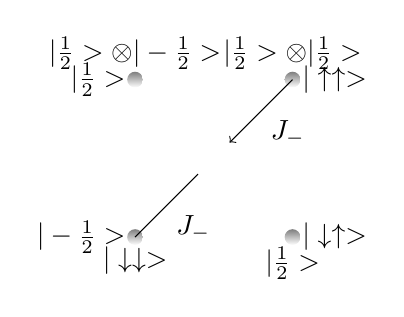
\begin{tikzpicture}
    \shade (-1,1) circle (.1)
     node [left] {$\ket|\frac12>$}
     node [above] {$\ket|\frac12> \otimes \ket|-\frac12>$};
    \shade (1,1) circle (.1)
     node [right] {$\ket|\uparrow\uparrow>$}
     node [above] {$\ket|\frac12>\otimes\ket|\frac12>$};
    \shade (-1,-1) circle (.1)
     node [left] {$\ket|-\frac12>$} node [below] {$\ket|\downarrow\downarrow>$};
    \shade (1,-1) circle (.1)
     node [below] {$\ket|\frac12>$} node [right] {$\ket|\downarrow\uparrow>$};
    \draw [->] (1,1) -- node [below right] {$J_-$} (.2,.2);
    \draw (-.2,-.2) -- node [below right] {$J_-$} (-1,-1);
  \end{tikzpicture}
\end{center}
The three $\ket|\uparrow\uparrow>$,
    $\frac1{\sqrt2}(\ket|\uparrow\downarrow> + \ket|\downarrow\uparrow>)$,
    $\ket|\downarrow\downarrow>$
are called the spin triplet, and the other single one is called the spin singlet.

We can take it into a grid
\begin{center}
  \includegraphics[width = \linewidth]{tensor}
\end{center}
By adding numbers to the vertical and horizontal side of the grid, there are
$(2j_1 + 1) \times (2j_1 + 1)$ intersections, with $j_1 + j_2$ irrep;
or a new rep from a new site to generate $j_1 + j_2 - 1$ irrep.
The states will eventually decompose to
\[
  j_1 \times j_2 = (j_1 + j_2) + (j_1 + j_2 - 1) + \cdots + |j_1 - j_2|.
\]

\section{Gauge}